\documentclass[border=2pt]{standalone}
\usepackage{tikz}
\usetikzlibrary{arrows.meta}

\begin{document}
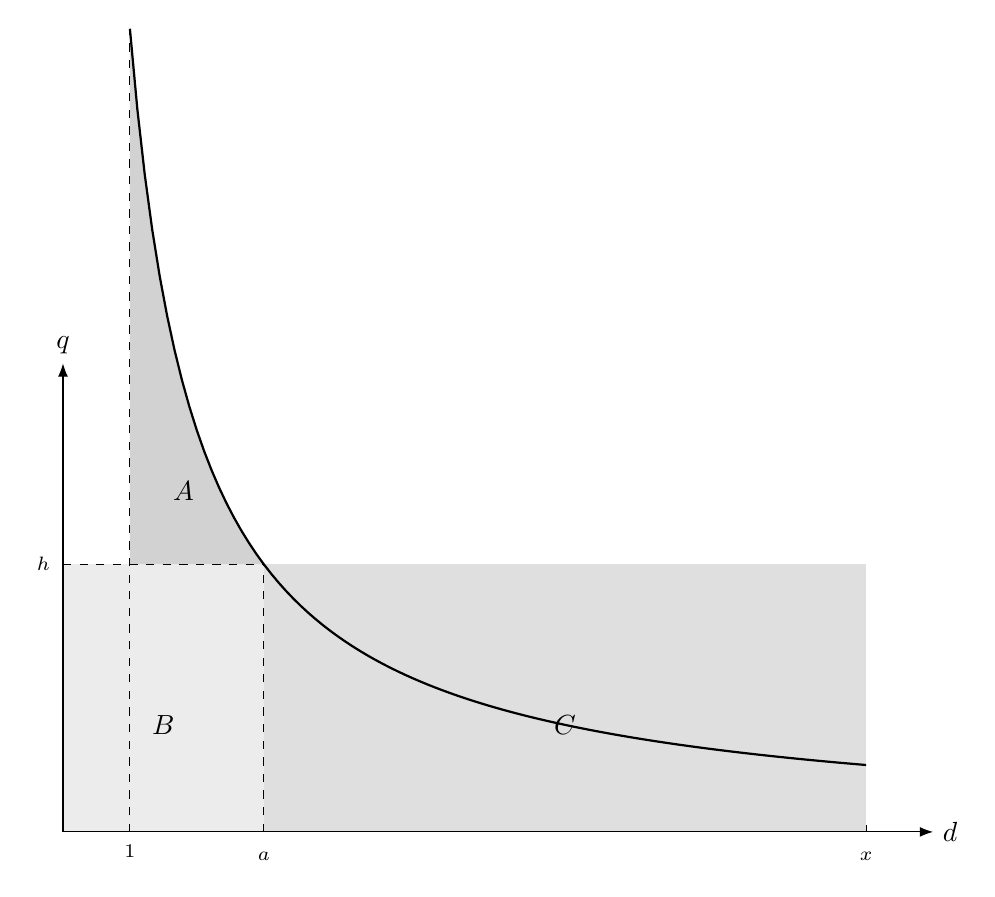
\begin{tikzpicture}[>=Latex, scale=0.85]

    % parameters: curve q = 12/d ,  a = 3,  h = 4  (so that a*h = 12 = x)
    \def\X{12}
    \def\A{3}
    \def\H{4}

    % region B: rectangle [0,a] x [0,h]
    \fill[gray!15] (0,0) rectangle (\A,\H);
    % region C: rectangle [a,x] x [0,h]
    \fill[gray!25] (\A,0) rectangle (\X,\H);
    % region A: under the curve, above h, from d=1 to a
    \fill[gray!35] plot[domain=1:\A,samples=60] (\x,{\X/\x}) -- (\A,\H) -- (1,\H) -- cycle;

    % axes
    \draw[->] (0,0) -- (\X+1,0) node[right] {$d$};
    \draw[->] (0,0) -- (0,7) node[above] {$q$};

    % curve q = x/d
    \draw[thick] plot[domain=1:\X,samples=100] (\x,{\X/\x});

    % dashed guide lines
    \draw[dashed] (0,\H) -- (\A,\H);
    \draw[dashed] (1,0) -- (1,\X);
    \draw[dashed] (\A,0) -- (\A,\H);
    \draw[dashed] (\X,0) -- (\X,0.1);

    % region labels
    \node at (1.8,5.1) {$A$};
    \node at (1.5,1.6) {$B$};
    \node at (7.5,1.6) {$C$};

    % axis ticks
    \node[below] at (1,-0.05) {\scriptsize $1$};
    \node[below] at (\A,-0.15) {\scriptsize $a$};
    \node[below] at (\X,-0.15) {\scriptsize $x$};
    \node[left] at (-0.05,\H) {\scriptsize $h$};

\end{tikzpicture}
\end{document}
